\documentclass[12pt, a4paper]{article}

\usepackage{preamble}

\title{Models of Associative Memory}

\author{Wenting Jin, Lucas Arnström \& Robin Eklind}

\begin{document}

\maketitle

\tableofcontents

\clearpage

% TODO: Add abstract?

% === [ Introduction ] =========================================================

\section{Introduction}

Associative memory may be defined as \textit{``the ability to correlate different memories to the same fact or event''} \cite{memristor_conditioning}. Two broad categories of associative memory distinguish between memory recalled from partial information or cues (auto-associative memory), and memory recalled from related categories or concepts (hetero-associative memory). To give an example, auto-associative memory is used when asked to fill in the missing parts (e.g. \textit{``Which country in Europe starting with an ``F'' is known as ``the land of a thousand lakes''?''}), while hetero-associative memory is used when asked what thoughts comes to mind (e.g. \textit{``If I say elephant, you may say pink, big or animal.''}).

% TODO: Add purpose, aim, and scope of the paper.

%\subsection{Hebbian Learning}

% ref: http://www.scholarpedia.org/article/Models_of_synaptic_plasticity
%
% (Hebb, 1949). The plasticity rule proposed by Hebb postulates that when one neuron drives the activity of another neuron, the connection between these neurons is potentiated.
%
% Theoretical analysis indicates that not only Hebbian like synaptic potentiation is necessary but also depression between two neurons that are not sufficiently coactive (Stent, 1973, Sejnowski 1977) Depression is necessary for several reasons, among them to prevent all synapses from saturating to their maximal values and thereby loosing their selectivity, and to prevent a positive feedback loop between network activity and synaptic weights.
%
% Phenomenological models are characterized by treating the process governing synaptic plasticity as a black box. The black box takes in as input a set of variables, and produces as output a change in synaptic efficacy. No explicit modeling of the biochemistry and physiology leading to synaptic plasticity is implemented.

% === [ Models of Associative Memory ] =========================================

\section{Models of Associative Memory}

\subsection{Hopfield Networks}

% Wenting.
Hopfield's model is an associative(content-addressable) memory model using binary information and its network is featured with threshold and feedback. A binary input vector to a Hopfiled Network will be recursively processed(fed back) at the granularity level of bit, until a threshold criterium is met, the produced output vector possesses the feature that is with the shortest Hamming distance to its origin input vector (see figure \ref{fig:hopfield_network}). There properties give rise to associative memory recall, where an input pattern (i.e. memory cue) is presented to the Hopfield network, which produces an output vector that is closest in Hamming distance to a previously stored memory, thus filling in the gaps to recall a memory through association.

\begin{figure}[htbp]
	\begin{center}
		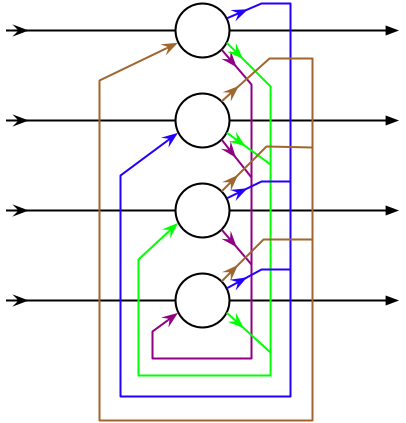
\includegraphics[width=0.5\textwidth]{inc/hopfield_network.png}
		\caption{A Hopfield network consisting of 4 nodes, with an input and output vector of length 4. Additionally, each node takes as input the state of each other node in the network.\protect\footnotemark}
		\label{fig:hopfield_network}
	\end{center}
\end{figure}
\footnotetext{Original image (CC BY-SA): \url{https://upload.wikimedia.org/wikipedia/commons/9/95/Hopfield-net.png}}

In paper from J.J.Hopfield(1982) \cite{computational_abilities}, the drawbacks of Perceptron were addressed through its intractable back-coupling, lack of abstraction properties and requirement of synchronism. Information storage was improved with help of Nonlinearity, and emergent computational properties were obtained from simple properties of many cells rather than complex circuitry(which is a result of linear associativity). The input-output relationship of nonlinear computation, binary threshold units and concept of the energy function were introduced.

Collective behaviors of the model was studied and resulted with the following findings: a few stable states was resulted from most of the initial state space, properties necessary for a physical content-addressable memory were not dependent on the symmetry of the connectivity matrix $T_{ij}$. Statement supported by findings from experiments is that "about 0.15N(memory storage bits, number of neurons) states can be simultaneously remembered before error in recall is severe", which refers to the memory capacity of the associative memory. Case with arbitrary starting state was studied and results of memories near to the starting state was highly produced. The nominally assigned memories which were called "attractors" dominates the phase flow whereas the flow is not entirely deterministic, which leads to a convergence to local optimum.

Case of consistent internal correlations in the memory was as well addressed, and Hebb synapses was used and slightly modified to generate nonsymmetric term~$\delta T_{ij}$, which limitation of sequence of four states was addressed.

\subsubsection{Implementation Example: Optical Information Processing}
In paper from D.Psaltis and N.Farhat(1985) \cite{optical_processing}, thresholding and feedback properties from Hopfield model was used in implementation of an optical system that processes optical information.

Enhanced error-correcting capability is one important outcome which is benefited from Nonlinearity of Hopfield model. With $M$ words of each binary vector $v_i$ with length of N bits, matrix $T_{ij}$ represents a storage of information. Matrix $T_{ij}$ gets multiplied by a stored binary vector $v'_i$ results in a \texttt{pseudoeigensystem} if $N$ is sufficiently larger than $M$. This indicated that the output vector $v''_i$ equals the input.

Supposed nonlinear iterative procedural experiments of certain number of known bits $N_1$ and the rest bits set to zero inside total of $N$ bits long vector were addressed to discover under what conditions the number of correct bits $N_2$ in output will be higher than $N_1$. A SNR(signal-to-noise ratio) equation which consists ratio of the expected value to the standard deviation on the same output vector, was used. As the Hopfield model has studied on the convergence property with respect to asynchronous operations, insensitivity to imperfections(nonuniformities, exact form of the threshold operation and errors in $T_{ij}$ matrix) and correct convergence obtained with thresholded $T_{ij}$. These all become most desired properties in optical implementation. Detailed optical implementation with 2D inputs was presented which was based on spatial-frequency multiplexing. Methods using Fourier transform, transmitting amplitude(weighted sum) and integral of the product of the input images were introduced in such an implementation. The robustness of a such system with nonlinear feedback becomes the most important feature.
As a conclusion, the implementation with the capabilities and limitations of optical techniques matches excellently with the Hopfield model that requires global, linear operations and local, point nonlinearities in a fully interconnected optical system.

\subsubsection{Memory Capacity with Modification: \\ replacing sigmoid neuron with a nonmonotonic neuron}
In paper from S.Yoshizawa, M.Morita and S.Amari(1992) \cite{capacity_of_nonmonotonic_model} it started with introduction of a new method by replacing sigmoid neuron with a nonmonotonic neuron and discussed theorectically on potential of absolute capacity(the maximum number of randomly generated patterns which are memorized as the equilibria of the network with the correlation-type connection weights) to be of order $n$ (nearly equal to $0.4n$).

Previous memory capacities were briefly introduced that Hopfield(1982) model's associative memory capacity is $0.15n$, the proven result of absolute capacity is asymptotically $ \frac{n}{2\log{n}} $ (from McEliece, Posner, Rodemich, \& Venkatesh, 1987; Weisbuch, 1985), and relative capacity(recalling process) is about 0.14n(with admission of small percent of errors) with replica method, but about $0.16n$ with a simply approximation method from respectively two different research work.

Various research suggestions were mentioned though all failed to deal completely with flaws of the conventional model, that both absolute and relative capacities are too small as well as the existence of large number of spurious memories. With a nonmonotonic neuron the result turned to be $0.4n$ for the absolute capacity which is even greater than relative capacity while the spurious memory disappeared.

With conventional neuron, memorized pattern is unstable, whereas a basin of attraction around memorized pattern was shown with nonmonotonic neuron by replacing sigmoid function with a nonmonotonic output function \textit{figure \ref{fig:nonmonotonic}} to neuron elements from the recalling process of an autocorrelation associative memory. This was named as Morita Model in the paper though it is essentially an extension from Hopfield Model.
By then the existence of equilibrium solutions and local stability, the authors did not further investigate on problems as the following: the size of the basin of attraction, the full sketch of spurious memories and the behaviour for clustered memorized patterns, which leaves more research work for future researchers to understand better associative memory with nonmonotonic neurons.

\begin{figure}[htbp]
	\centering
	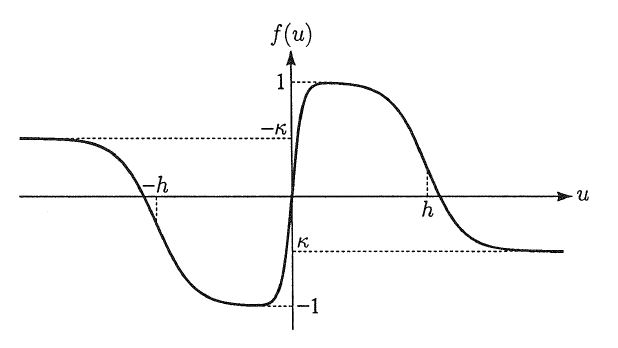
\includegraphics[scale = 0.8]{inc/nonmonotonic.jpg}
	\caption{The nonmonotonic output function, S.Yoshizawa, M.Morita and S.Amari(1992)}
	\label{fig:nonmonotonic}
\end{figure}

%THIS IS STH EXTRA OUTSIDE HOPFIELD
\subsection{Experiment on Implicit Memory for Novel Associations between pictures: \\ Effects of Stimulus Unitization and Aging\cite{stimulus_unitization_and_aging}}

From various previous research, concepts such as associative priming, unitization, difference between conceptual and perceptual associative priming, verbal versus pictorial material/stimuli and roll of spatial proximity were briefly summarized.


Experiments with pictorial stimuli(paired pictures) were done in 3 consecutive stages, where the result from first stage showed no evidence on requirement of spatial contiguity, though associative priming was enhanced compared to with spatially separated stimuli, which proved "implicit memory for novel associations still can occur in the absence of an emergent conceptual representation". The second experiment was an extension from the first experiment, with focus on the effects of aging and spatial contiguity of the same topic of stimuli on novel association priming between pictures, where stunning result was shown that "associative priming is age invariant"(exposure of pictures was longer with older group to yield a matched performance in the baseline). The last experiment was based on both first and second experiments that "associative priming with pictorial stimuli is modulated by spatial contiguity but not by aging", and the study proved further evidence for the notion that novel association priming for picture pairs is mediated by the PRS(Perceptual Representation System).

\subsection{Boltzmann Machine}

% --- Lucas

\begin{figure}[htbp]
	\begin{center}
		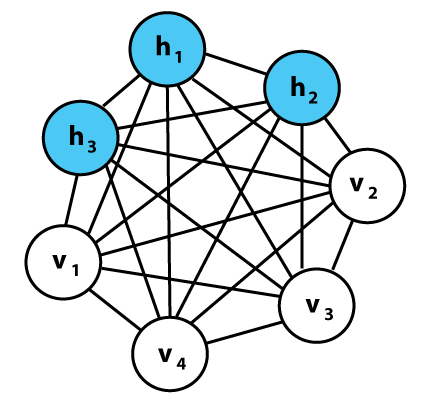
\includegraphics[width=0.5\textwidth]{inc/boltzmann_machine.png}
		\caption{Illustration of a Boltzmann Machine. The blue units represents three hidden units, while the four white units represents four visible units.\protect\footnotemark}
		\label{fig:boltzmann_machine}
	\end{center}
\end{figure}
\footnotetext{Original image (Public Domain): \url{https://en.wikipedia.org/wiki/File:Boltzmannexamplev1.png}}

The "Boltzmann Machine" (BM) is a form of "parallel constraint satisfaction network" \cite{ackley1985learning}. It is capable of learning the underlying constraints of a domain by only being shown examples of it. The BM is composed of units forming a complete graph where the connection between two units are symmetric, meaning that the weight on the connection is the same in either direction. No unit has a connection to itself. The units are binary, meaning that they can assume one of two states, on or off. The state of a unit is determined by a probabilistic function based on the states of the units neighbours. A strong connection (high weight value) between two units indicates that if either of these two units are active, the other one should probably be active as well. While a weak connection (low weight value) indicates that these should probably not be active at the same time.

The BM is notably similar to the Hopfield network in that it also defines a global energy state of the system, utilizing the same equation that determines the global energy value. Each global state can be identified by the energy of the system in that state. By forcing the values of the visible units to represent a training set the system attempts to find an energy configuration that is compatible with the given input. The resulting energy state can then be interpreted as to how well the given data fulfils the constraints of the domain. Thus by minimizing the energy the system learns an interpretation of the problem that increasingly satisfies the constraints of the domain.

The simplest way to minimize the energy into a local minimum of the system is to change each unit into a value that results in a lower energy state. The data needed to determine this change is locally accessible to each unit. If the sum of all values for a given units neighbour exceeds the threshold of that unit, the resulting state of the unit should be on. Otherwise it should be off. This is the usual algorithm for binary units.

Because of this deterministic algorithm it suffers from the usual weaknesses of gradient descent algorithms, namely it gets stuck in local minima if its initial state is close to one. In order to alleviate the algorithm of this problem noise is introduced in the training. This allows the network to "jump" out of these minima into configurations of higher energy. The algorithm used for noise introduction is a variation of the "Metropolis algorithm" \cite{metropolis1953equation} that was used to study thermodynamic systems. This modified version introduces a concept of temperature to the machine. The machine then tries to reach "thermal equilibrium" during training. Meaning that the machine is allowed to run repeatedly until the global energy of the system converges to a fixed state over a temperature that is initially high and then slowly decreased over the runtime of the system. The probability of finding the system in a global state after it has reached thermal equilibrium follows a Boltzmann distribution.

%TODO write more about this temperature thing
%TODO write more about the probabilistic features of the BM as well as the boltzmann distribution that gives the system its name.

Training is conducted in two phases, in the first phase the visible units of the machine are set to the values of the training set. In the next phase the machine is allowed to run freely, independent of the training set. The machine is iteratively switched between these two phases for the duration of the training until it reaches thermal equilibrium. The goal of the training is for the machine to generate the input vector with a high probability.

% --- NOTES
%The difference between the BM and the Hopfield network is mainly that the nodes (or units as they are referred to in the original paper) of the Boltzmann Machine are stochastic by nature.
%The BM can be used for constraint satisfaction problems that involve a large amount of weak constraints.

\subsection{Memory Resistor}

%Robin.

Memory resistors, memsistors for short, are passive circuits which change their resistance as current flows through them, and maintain their resistance in between use. In other words, memsistors remember past flows of current (i.e. store state), and control resistance based on this knowledge (i.e. stored state). Several similarities have been identified bewteen the properties of memsistors and synapses, which make them interesting candidates for associative memory models.

TODO: Extend. Artificial synapses experiment using memsistors conducted in 2010, empiricially validating the formation of associative memories using three neurons and two synapses \cite{memristor_conditioning}.

TODO: Extend. The memsistor was hyphosized in 1972 by Leon Chua, the father of non-linear curcuit theory, who presented it as the missing fundamental cirtuit element (see figure \ref{fig:circuit_elements}) \cite{chua_memristor}. Looking at the current~$I$ and voltage~$V$ plot, a memsistor may be identified by the pinched hysteresis loop going through origo (see figure \ref{fig:pinched_hysteresis}. TODO: Explain the underlying reason of the hysteresis loop, i.e. alterating between two states (metastable switch).

% ref: Finding the Missing Memristor - R. Stanley Williams
%
% > The fourth fundamental passive circuit element.
% >
% > Resistor
% > Capacitor
% > Inductor
% >
% > AND Memristor
% >
% > UC Bercley Lean Chua is to circuit theory what Albert Einstein is to relativity.
% > The father of non-linear cirtuit theory.
% >
% > Noticed something missing from the circuit diagram; based on symmetry and beauty, there should be a fourth.
% > Original paper, memsitory the missing circuit element. 1971
% >
% > Passive device with state.
% >
% > Frequency response of Lissajous figures.
% > The pinched hysteresis loop.
% >
% > "If you see a pinced hysteresis loop in an IV-curve, you've probably got a memristor."
% >
% > Make a circuit using only resistors, capacitors and inductors to come up with the IV-characteristics of a memristor. It cannot be done, and thus belongs to it as a fundamental device; as proven by Lean Chua.
% >
% > Even before the original paper in 1971, there was peer-review research published which illustrated pinched hysteresis loop. Basically they had managed to discover the memristor, they just didn't know what it was called and thought it was an abnomality.
% >
% > Strukov, Stewart, Snider & Williams, Nature 453 80 (2008)

\begin{figure}[htbp]
	\begin{center}
		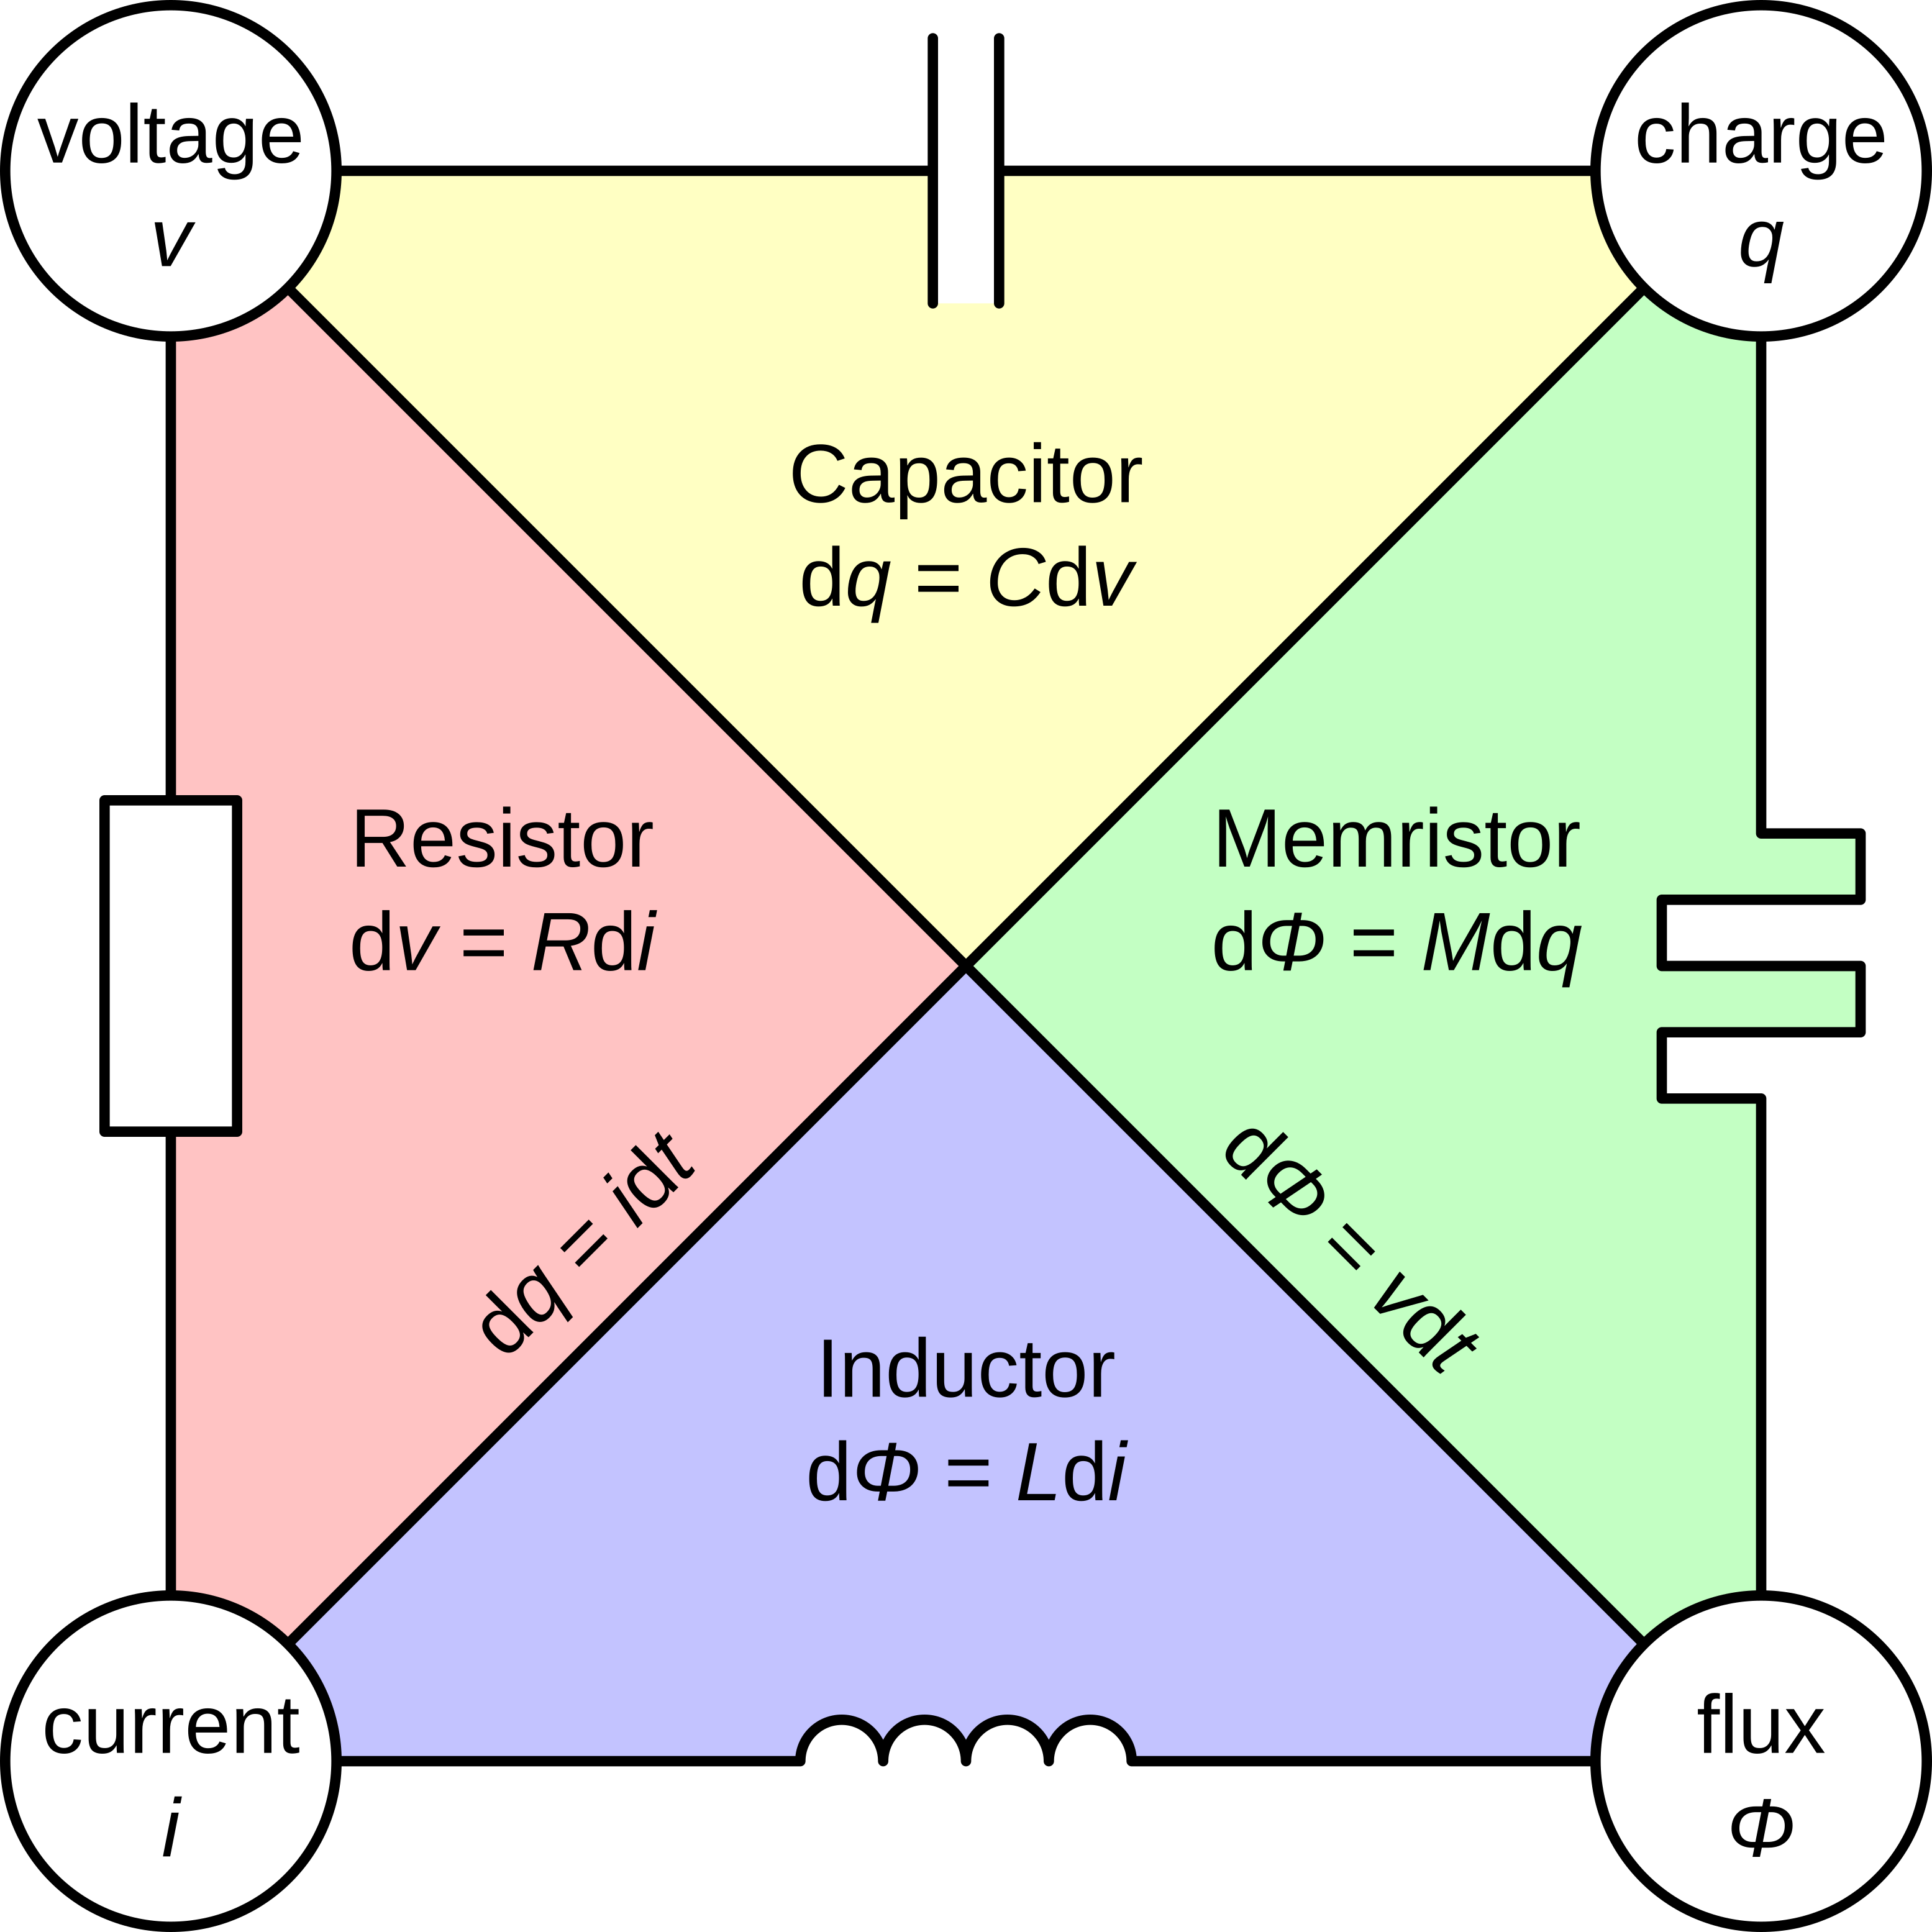
\includegraphics[width=0.5\textwidth]{inc/circuit_elements.png}
		\caption{Fundamental circuit elements.\protect\footnotemark}
		\label{fig:circuit_elements}
	\end{center}
\end{figure}
\footnotetext{Original image (CC BY-SA): \url{https://en.wikipedia.org/wiki/File:Two-terminal_non-linear_circuit_elements.svg}}

\begin{figure}[htbp]
	\begin{center}
		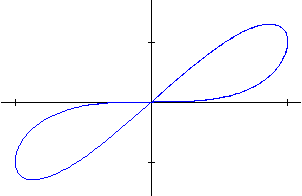
\includegraphics[width=0.5\textwidth]{inc/pinched_hysteresis.png}
		\caption{A pinched hysteresis loop plotted on an IV-curve.\protect\footnotemark}
		\label{fig:pinched_hysteresis}
	\end{center}
\end{figure}
\footnotetext{Original image (CC BY-SA): \url{https://en.wikipedia.org/wiki/File:Pinched_crossing_hysteresis.png}}

TODO: Extend. In 2008, HP released a paper titled \textit{The missing memristor found}, which outlined the hardware implementation of a memsistor \cite{hp_memristor_found}, thus validating the existence of the hypothesized memsistors circuit element. Retrospectively, several research groups had discovered circuits with the tell-tale properties of memsistor, i.e. with a pinched hysteresis loop. TODO: Include ref about prior research, before 2008.

% ref: Tim Molter HiPeac Prague 2016 Memristor Keynote
%
% The resistance of a memristor depends on the history of current that has previously flowed through the device.
%
% Search for "memristor" on Google scholar has been doubling every 18-24 months since 2008.
%
% Down to 50 Angstroms device size theoretically possible.
%
% Denser memory, faster read and write, lower energy use, non-volitile, and may represent continuous (i.e. not 0 and 1).
%
% How do we reach the power efficiency of a brain. "Don't simulate a brain, build a brain"
%
% We need to build a brain where the distance between memory and computation is 0.
%
% 1 billion fold discipancy between current machine learning platforms and biological brains.
%
% We can operate on very low voltages because of the read and write phases that constantly repair relevant state.

% ref: Knowm Collaborates with Kris Campbell at BSU
%
% Continous value stored as resistance in a memristor. breaking outside of the 0 and 1 box.

% ref: http://knowm.org/
%
% > ## Modern computing
% >
% > Clear distinction between memory and processing.
% > Shuttle information back and forth.
% > Takes too long, requires too much energy.
% >
% > ## New paradigm of computing
% >
% > The act of accessing memory is the act of processing.

% ref: https://www.youtube.com/watch?v=Tb2E-t11OH4 ("What is AHaH Computing?")
%
% > Large scale adaptive learning systems, like brains.
% >
% > Bring memory and processing closer together. Parallel computing.
% >
% > Reduce or eliminate the energy normally associated with computing those functions.

% ref: https://www.youtube.com/watch?v=IVDRcV8XvlI ("What is an AHaH node?")
%
% > Two memristors competing with each other.
% >
% > A kT-bit (thermodynamic bit), a synapse consisting of two memristors.
% >
% > Look at the leaf of a plant. Energy dissipating system, constructed of many bifircating channels. Every place where the energy flow splits, you have an AHaH node. You have two competing energy dissipating pathways.
% >
% > Nature is built of AHaH nodes.
% >
% > Understand how things self-organize.

% ref: https://www.youtube.com/watch?v=R7HxFhVQVr4 ("Why AHaH computing?")
%
% > Current digital computing platforms are billions of times less power and space efficient than biology (brains) for synaptic operations.
% >
% > It's physically not possible to reach biological level efficiency without significant changes in both architecutre and technology.
% >
% > "GPU's will save us." `No they won't, they just suck less`
% >
% > If you insist on separating memory and computing, you won't even get close to the capacity of biology.
% >
% > Traditional computing would go an inch while biology is able to circle the world.
% >
% > Effective intelligence.

% ref: https://www.youtube.com/watch?v=YOKr8n6Juhs ("Why is AHaH computing so efficient?")
%
% > Communication is way faster in technology than biology. 1sec football field, 1sec 7 times around the world.
% >
% > Neuron body: 4000-100 000nm
% > Synapses: 500 nm
% > Viruses: 400-40 nm
% > Transistor: 28 nm
% >
% > If faster and smaller, why so inefficient?
% >
% > Currents naturally sum. The values are reduced to specific resistances.
% >
% > Memristor
% >
% > Measures the combined current.
% >
% > Memristors can radically reduce total communication distance for some problems (not all).
% >
% > Reduce voltage makes a big impact, since it's the voltage squared.
% >
% > E=(C*V^2)/2
% >
% > biology: 0.065V
% > computer: 1.2v (18x biology) 18^2 -> 324.
% >
% > Reduce the communication distance and voltage.

% ref: https://www.youtube.com/watch?v=ZBJX6zzwnRI ("The Adaptive power problem.")
%
% > Noise is everywhere.
% >
% > Noise margin (analog vs digital).
% >
% > The signal gets corrupted by the noise.
% >
% > Memristors. Two meta-stable switches. Potential energy that has to be overcome to have a transition.
% >
% > We want: Low power + adaptation ("ability to change")
% > But: Parts will constantly break (because of noise), decay, volitility
% > Consequently: We need a mechanism of repair.
% >
% > The Adaptive Power Problem
% > Low Power + Adaptation = Parts break
% >
% > Intelligence -> Learning -> Adaptation

% ref: https://www.youtube.com/watch?v=NO9kmqr8NLk ("The Adaptive Power Solution")
%
% > Intrinsic mechanism of repair; inherent.
% >
% > What if constant adaptation *is* the mechanism of repair?
% >
% > What is the "essential nature" of adaptation?
% >
% > When nature minimizes its potential energy, it also solves our problem."; e.g. minimal surface with soap bubbles.
% >
% > To repair yourself is to be alive. Death is decay.
% >
% > Bejan (Construcal Law):
% > "For a finite-size system to persist in time (to live), it must evolve in such a way that it provides easier access to the imposed currents that flow through it."
% >
% > Swenson:
% > "A system will select the path or assembly of paths out of available paths that minimizes the potential or maximizes the entropy at the fastest rate given the constraints."
% >
% > England:
% > "Dissipation-driven adaptation of matter."
% >
% > E.g. The system will go with the flow, and it will maximize the flow.
% >
% > Maximize the dissipatation of energy. The system will evolve in time towards that maximum, intrinsic repair.
% >
% > Have the system evolve itself to solve our problems.
% >
% > AHaH circuit. An intrinsic adaptation mechanism. Energy dissipation pathways competing for conduction resources.
% >
% > Everywhere in nature. Competing energy dissipating pathways. Fractal.
% >
% > A memristor is effectively an adaptive energy dissipating pathway. It's like a riverbed. As you pass current through it, it will change its resistance, the riverbed will get bigger. Make memristors compete for energy dissipation.
% >
% > AHaH - Anti-Hebbian and Hebbian plasticity
% >
% > "Maximization of energy dissipation" - Swenson
% > "Maximization of currents" - Bejan
% > "Dissipation-driven adapataion of matter" - England
% > "Energy dissipation pathways competing for condution resources" as a mechanism.

% ref: https://www.youtube.com/watch?v=CFSrC7kjbJo ("Introduction to AHaH Computing, Alex Nugent, RIT, April 2015")
%
% > Focuses on self-organizational building blocks.
% >
% > Points of bifercation, branches.
% >
% > Energy dissipating fractal pattern.
% >
% > d (the distance) is zero in the brain, has tremendous effects on energy usage.
% >
% > "If it's pinched it's a memristor"
% > - Leon Chua
% >
% > Plot voltage vs current. You get this pinched hisorises loop. Implies that the device has a memory. If it was just a resistor it would be a line. If it was a capacitor it would be a circle.
% >
% > Tell tale sign that it is a memristor.
% >
% > A memristor for each pathway, and they are competing with eachother so you need two per synapse. Think of the pair as a synapse itself, and the different in conductance between the two is the value of the synapse. If one is more conductive than the other it is positive, and vise versa, its negative.
% >
% > Naturally they go towards zero. But if you give them a burst, you can make them positive or negative as you want. Read brings it a little closer together, then reward it.
% >
% > Hebbian (erase the path): Any modification to the synaptic weight that reduces the probability the synapic state will remain upon subsequent measurement.
% >
% > Anti-hebbian (select the path): Any modification to the synaptic weight that increases the probability the synaptic state will remain the same upon subsequent measurement.
% >
% > XXX [ IMPORTANT ] XXX
% >
% > Synaptic access is processing is adaptation (memory and processing merged, d=0).
% >
% > XXX [/ IMPROTANT ] XXX
% >
% > A neuron is this decision making thing. We are finding the decision boundry, a representation of the weights w_0, w_1.
% >
% > Maximize the classification margin.
% >
% > Opposing data distribution (energy dissipation pathways)
% > fight for classification margin (compete for conduction resources)
% >
% > Spike encoding (optic nerve). Which spikes within the spike space are active.
% >
% > FF-RF (forward-float, reverse-float), that is the as close to non-destructive read as you get. Reading is adaptation, it changes the memory.
% >
% > We can go backwards, discretized by the spikes.
% >
% > Nature has a universal adaptive building block.
% >
% > Interacting collectives of this builing block solves the problems that the brain solves.
% >
% > memristors empower (not replace) our digital computers.

% ref: https://youtu.be/dgbooumJ4Tg?t=1692
%
% Won a nobel price. Eliol Prigoge.
% There is a natural tendency for complex systems to minimize the energy consumption

\subsubsection{Knowm Synapses}

% ref: http://knowm.org/knowm/
%
% A memristor is the electronic equivalent of an adaptive container!
%
% “Anti-Hebbian and Hebbian” in honor of Donald O. Hebb
%
% “Knowm’s Synapse” or “Nature’s Transistor”. Two competing energy dissipation pathways.
%
% As a voltage (pressure) is applied to a memristor, its conductance will change.
%
% It is responsible for most self-organization on this planet. Nature is built of Knowms, including you.
%
% It is created when two energy dissipation pathways are competing for conduction resources. It appears to be at the heart of most self-organization.
%
% Knowm is built of a simple part repeated over and over again.
%
% When energy (for example water) flows through an adaptive container (for example dirt), the medium adapts or erodes in a particularly way that causes the energy to be dissipated faster. For example, the water erodes the ground and causes a channel to grow, which lowers the resistance to flow.
%
% ref: http://knowm.org/knowm-api/
%
% Every modern computing system currently separates memory and processing. This works well for many tasks, but it fails for large-scale adaptive systems like brains or large ML models like neural networks. Indeed, there is no system in Nature outside of modern human digital computers that actually separates memory and processing, so it’s a wonder we have been able to do as much as we have.

% ref: ref: http://knowm.org/report-from-the-navy-karles-invitational-on-neuro-electronics/
%
% Where each operation results in Anti-Hebbian or Hebbian learning. At the lowest level, Anti-Hebbian just means “move the synapse toward zero” and Hebbian means “move it away from zero”.

% === [ Current Capabilities ] =================================================

\section{Current Capabilities}

TODO: Define capabilities in terms of capacity and applications.

%Definitions of capacity.
%
%\begin{itemize}
%\item Absolute capacity.
%\item Relative capacity.
%\item Capacity of associative memory
%\item Relative capacity of recalling process
%\end{itemize}

\subsection{Hopfield Network}

TODO: Move applications and capabilities of Hopfields from the Model section to this section.

%Wenting.

1982, $0.15n$ (capacity of associative memory)

% Above 0.15n releases the constraint on symmetries according to Olle.

1985, proven $ \frac{n}{2\log{n}} $ (absolute capacity)

1985, $0.14n$ (relative capacity of recalling process)

1993, $ n ~= 0.4n $ (new result, absolute capacity)

\subsection{Boltzmann Machine}

%Lucas.

\begin{figure}[htbp]
	\begin{center}
		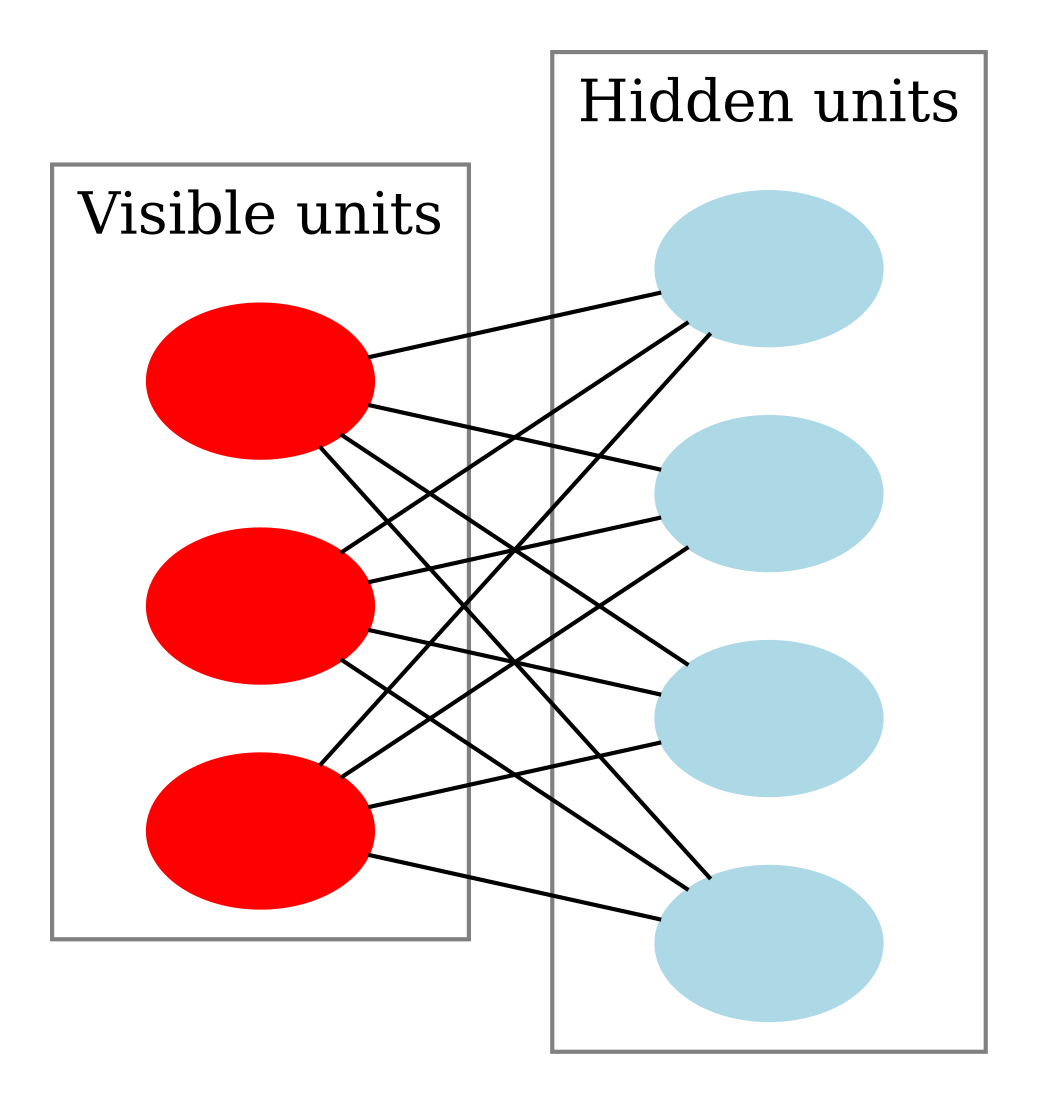
\includegraphics[width=0.5\textwidth]{inc/Restricted_Boltzmann_machine.png}
		\caption{Illustration of a Restricted Boltzmann Machine.\protect\footnotemark}
		\label{fig:restricted_boltzmann_machine}
	\end{center}
\end{figure}
\footnotetext{Original image (CC BY-SA): \url{https://en.wikipedia.org/wiki/File:Restricted_Boltzmann_machine.svg}}

Unfortunately, the Boltzmann Machine is slow to train and is thus only practical for simpler problem domains. If the BM is scaled beyond any trivial domain it becomes too slow and almost stops learning. This is due to the fact that all units of the BM are fully connected to each other which does not scale well.

In order to use the BM for bigger tasks a restriction has to be made. Namely, connections between units in the same layer can not be allowed. This is called the Restricted Boltzmann Machine (or "Harmonium" as the original author referred to it) \cite{smolensky1986information}.

Versions of the Restricted Boltzmann Machine (RBM) have been successfully used in many applications such as deep learning \cite{hinton2012better} and speech recognition \cite{dahl2010phone}.

The general idea when using RBM's in deep learning is to "stack" several RBM's on top of each other. The activities of the units in the hidden layer of one RBM can be used as input vector for an other RBM. This way the overall system does not have the problem with scalability that the ordinary Boltzmann Machine suffered as well as the added bonus that the generative model is improved each time a new layer is added on top of the existing ones.

\subsection{Memory Resistor}

%Robin.

Proof of concept in 2010, using 3 neurons and 2 synapses to achieve 1 associative memory formation.

%ref: http://www.hpl.hp.com/news/2008/apr-jun/memristor.html
%
% > "The memristor could lead to far more energy-efficient computers with some of the pattern-matching abilities of the human brain.
% > - Jamie Beckett, April 2008

% === [ Future Potential ] =====================================================

\section{Future Potential}

% ref: Connectome.
%
% 100 000 000 000 neurons
%
% 10 000 more synaptic connections

% ref: https://www.youtube.com/watch?v=JqMpGrM5ECo (The Human Brain Project - Video Overview)
%
%     100 000 000 000 neurons
% 100 000 000 000 000 synapses


\subsection{Intelligent Systems}

Intelligence defined by ability to make predictions, not behaviour \cite{intelligence_is_prediction}.

% ref: http://knowm.org/the-constraints-for-neuromorphic-computing-systems-have-suddenly-changed/
%
% In almost every machine learning algorithm or program, there lies an equation that looks something like this:
%
% w_{t+1}=w_{t}+\delta w
%
% In other words, the weight is nudged a bit. Sometimes it’s nudged in a positive direction. Sometimes it’s nudged in a negative direction. Sometimes it’s a big nudge. Sometimes it’s a small nudge. Most of machine learning boils down to understanding how to nudge weights around.
%
% The space of possible memristors is enormous and most of them don’t work exactly how we want them too. Some are too stochastic (random). Some do not switch quickly enough, or they switch too fast. Some are not bi-directional (meaning that we can’t controllably increase and decrease the resistance via the applied voltage direction). Many memristors are not incremental, meaning that their resistance can only be changed in large steps. Others are only incremental in one direction and will abruptly change in the other direction. Still others will stop working after only a few thousand switching events. Indeed, when one stops theorizing and goes out to find a suitable memristor–things get very difficult very quickly!
%
% `It now seems clear that a capacity to learn would be an integral feature of the core design of a system intended to attain general intelligence, not something something to be tacked on later as an extension or an afterthought`
% - Nick Bostrom, “Superintelligence: Paths, Dangers, Strategies”
%
% Artificial General Intelligence.

\subsection{Energy Efficiency}

Network in its true sense, \textit{the net is doing all the work} \cite{net_doing_all_the_work}.

\cite{ahah}

%Current computer architectures are designed around major bottlenecks, huge amounts of data has to be shuffled back and forth to perform computations. Reaching its limits; transistors now so small that they only allow a single electron to pass through (similar in size to the ion channels). At this scale, problems arise when transistors may allow electrons to pass through, when they shouldn't and wise versa; which leads to unpredictable behaviour (small bursts of ones when should be be all zero, and wise versa.)

%The brain, parallel, error correcting, memory efficient. (not doing a lot of unnecessary data shuffling?)

% ref: From BrainScales to Human Brain Project Neuromorphic Computing Coming of Age
%
% Human Brain Project.
%
% 50 000 000 synapses, and about 200 000 neurons
%
% 10 000 faster than biological real-time.
%
% Performance.
%
% 10 femtojoul
%
% 1 joul (in super computers) 10^14
%
% Physical models (neuromorphic)
%
% 10 000 000 times more energy efficient than the state-of-the-art HPC (comparable model)
%
% 10 000 less energy efficient than biology.
%
% Including all the overheads.
%
% # Time Scales
%
% Causality detection   | 10^{-4} sec | 0.1 sec          | 10^{-8} sec |
% Synaptic plasticity   | 1 sec       | 1000 sec         | 10^{-4} sec |
% Learning              | 1 day       | 1000 day         | 10 sec      |
% Development           | 1 year      | 1000 year        | 3000 sec    |
%
% 12 orders of magnitude
%
% Evolution             | > millenia  | > 1000 millenia  | > months    |
%
% > 15 orders of magnitude

%# Applications
%
% Reverse engineer biological data

% ref: Schmuker, Michael, Thomas Pfeil, and Martin Paul Nawrot. "A neuromorphic network for generic multivariate data classification."
%
% TODO: Check :) HBP Roadmap for 2023
%
% Spikey (Heidelberg Lab), commercially available.
% 384 neurons
% 100 000 plastic synapses
% 10.000 - 100.000 real-time
% put and pray into Laptop with USB.
%
% Neuromorphic computing
% Consistent concept for non-von Neumann, non-Turing computer architecture.
%
% Watch the market for Resistor memory, once it is there they will use it for HBP, but using CMOS for now, similar to how von-Neumann used Vaccum tubes before the arrival of the transistor.

% ref: http://knowm.org/how-to-build-the-ex-machina-wetware/
%
% Once you understand what is going on, you can start to understand how to harness it. Think about it. If a bunch of particles will spontaneously organize themselves out of a colloidal suspension to dissipate energy then what happens when we control the energy? What happens if we make the maximal-energy-dissipation solution the solution to our problem? Will the particles self-organize to solve our problem? The answer, it turns out, is a resounding “yes”.
%
% Find a way to use nature as nature itself does. To not compute a brain, but to actually build one. To find a way for matter to self-organize on a chip to solve computational problems.
%
% Memory and processing merge, voltages and clock-rates drop and power efficiencies explode.
%
% AHaH Computing is about understanding how to build circuits that adapt or learn to solve your problems and, as a result, dissipate more energy ‘as a reward’. The path to maximal energy dissipation is the path that solves your problem, and the result is that Nature self-organizes to solve your problem.

% ref: http://knowm.org/the-gordon-panthana-dialog/
%
% It of course does not mean you can magically make a circuit that consumes zero energy. It means that calculation of very large numbers of interacting adaptive variables via the separation of memory and processing is overwhelming less efficient than building a very large interacting adaptive system directly. The example was meant to show just how significant this contribution can be, and why having an intrinsically adaptive element (the memristor) is exciting and useful.
%
% Specifically we use the physics of memristors to eliminate the power and time normally associated with synaptic integration and adaptation.
%
% AHaH Computing embraces hardware as part of the solution and designs from the bottom-up (hardware) and top-down (AHaH compatible algorithms). The result is a broadly commercially viable machine learning system that can scale to biological levels of efficiency.

% ref: http://knowm.org/report-from-the-navy-karles-invitational-on-neuro-electronics/
%
% Dr. Kwabena Boahen
%
% Comparing the scaling problem of CMOS transistors to traffic. He showed that as CMOS transistors are scaled down, and the number of electron ‘lanes’ get close to one, the devices exhibit extremely high magnitude noise due to individual electrons becoming trapped in local energy minima (pot holes) and blocking the traffic. In essence, when the transistors are large, any “stuck electrons” are easily bypassed and their contribution to the total current is minimal. However, when the devices approach the natural ‘lane width’ of an electron (about 2.7 nm if a remember correctly), a stuck electron could reduce the current by 50% or even shut down the whole device. The answer to these problems, Dr. Boahen believes (and I agree), lie in distributed fault-tolerant analog architectures inspired by the brain.

%\subsection{Independent Component Analysis}

% ref: http://knowm.org/report-from-the-navy-karles-invitational-on-neuro-electronics/
%
% Dr. Marcel Adam Just
%
% For example, when somebody thinks about an “orange”, for example, their brains activate representations for a color, and a shape, and a fruit, and other associations. By identifying these “thought components” and using machine learning, they can predict with high accuracy what object the person is thinking about. They have gone further with this, decomposing human emotion into a “basis set” of three components that they call “Valence” (is it good or bad), “Arousal” and “Social Interaction”.
%
% What really surprises me is that the exact same places of a brain are active for the same abstract concepts from one person to the next. That is, when I think of an “orange” and parts of my cortex light up corresponding to shape, color, texture, etc…the exact same places in your brain light up to represent the same abstract concepts! It would appear that while the human brain must learn these concepts, the location for where the learning occurs is genetically determined.

% === [ Conclusion ] ===========================================================

\section{Conclusion}

All three models make use of Hebbian learning. TODO: Extend.

% === [ Research Literature ] ==================================================

Preliminary list of references, cited to force inclusion within the bibliography.

% TODO: Add to this list throughout the project.

% Wenting
\cite{computational_abilities} \cite{optical_processing} \cite{capacity_of_nonmonotonic_model} \cite{stimulus_unitization_and_aging}

% Lucas
%\cite{ackley1985learning} \cite{capacity_of_hopfield} \cite{high-order_neural_networks} \cite{neural_network_models_for_associative_memory} \cite{sparsely_encoded_associative_memory}

% Robin
\cite{memsistor} \cite{principle_of_neural_associative_memory} \cite{parallel_models_of_associative_memory} \cite{associative_memory_using_small-world_architecture} \cite{associatron} \cite{associative_search_network} \cite{deep_machine_learning} \cite{on_associative_memory} \cite{from_cell_to_cortex} \cite{ahah}

\bibliography{references}

\end{document}
